\documentclass{article}

\usepackage{tikz}
\usepackage{geometry}
\usetikzlibrary{positioning}
\geometry{left=1.0cm} 
\usetikzlibrary{automata,positioning,arrows,chains,shapes}

\begin{document}

	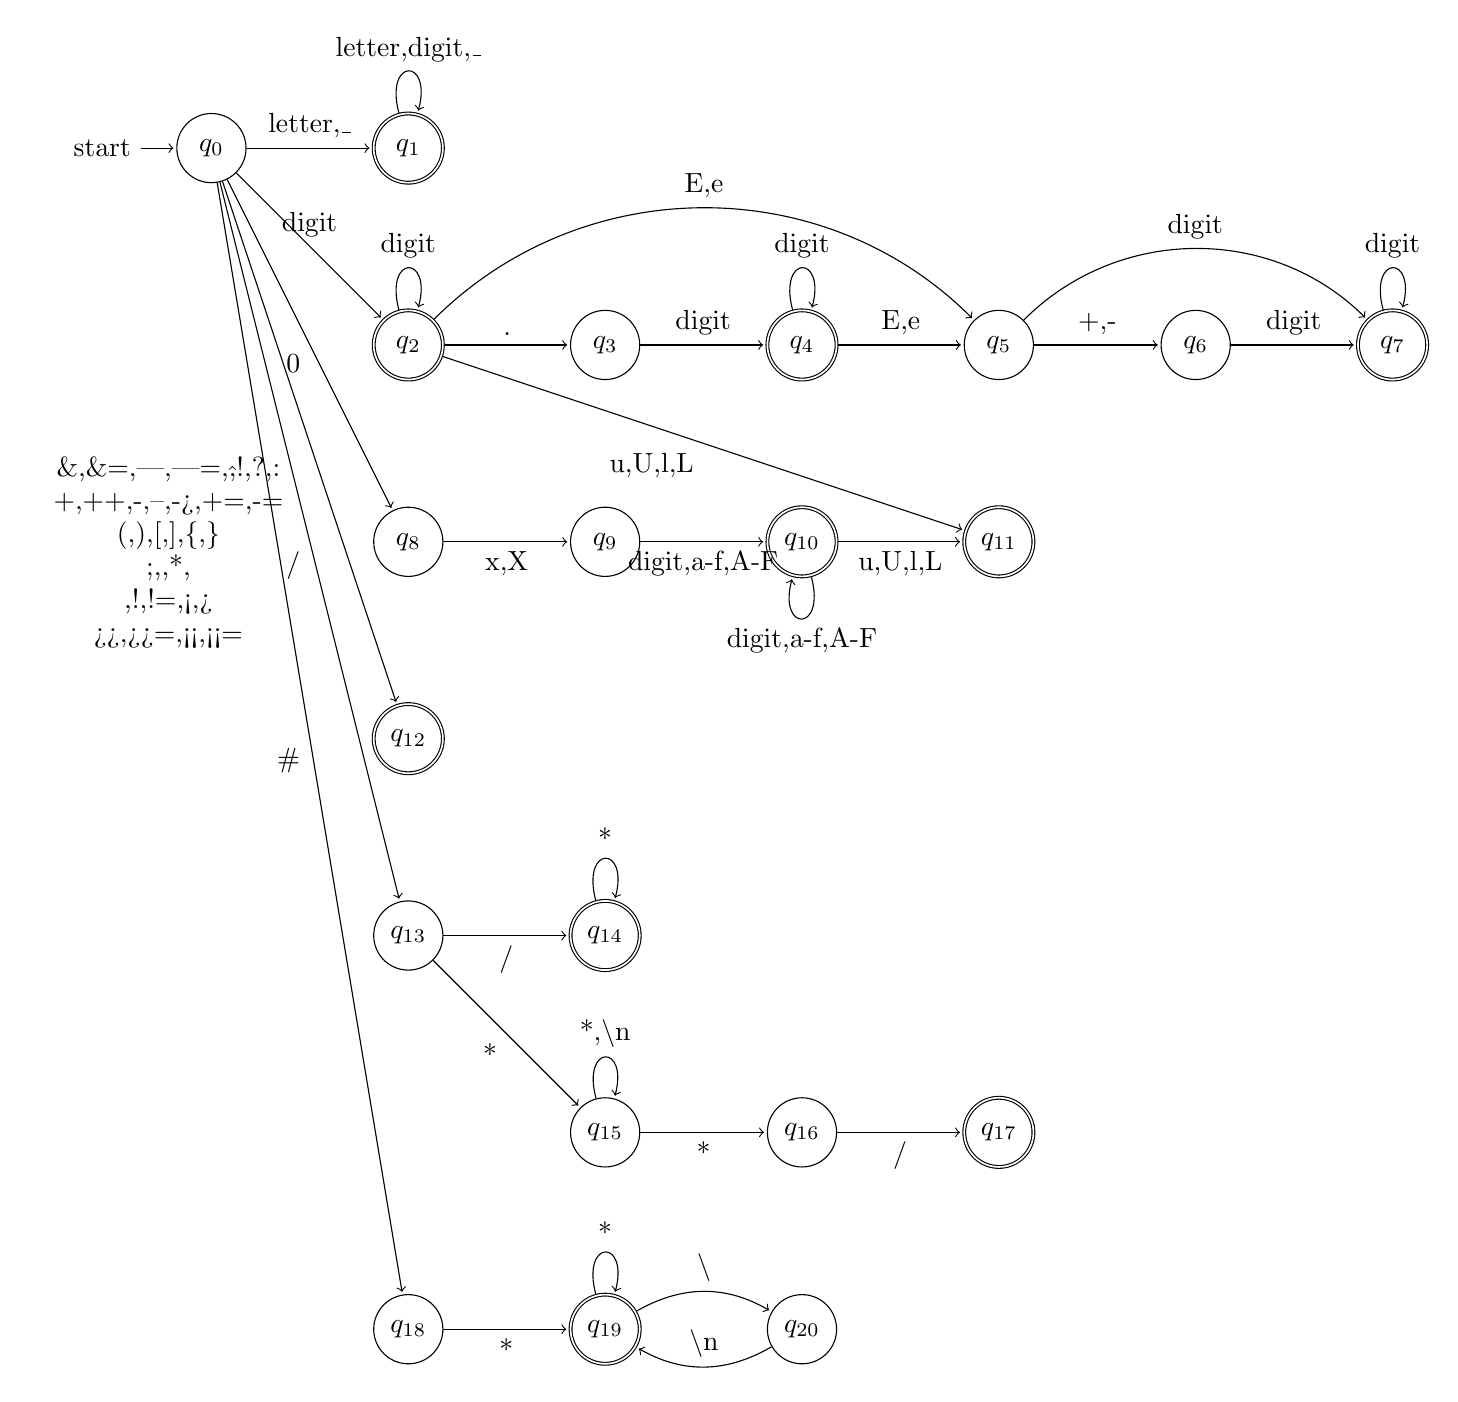
\begin{tikzpicture}[shorten >=1pt,node distance=2.5cm,on grid,auto] 
		\node[state,initial] (q_0)   {$q_0$}; 
		\node[state,accepting] (q_1) [right=of q_0] {$q_1$}; 
		\node[state,accepting] (q_2) [below=of q_1] {$q_2$}; 
		\node[state] (q_3) [right=of q_2] {$q_3$}; 
		\node[state,accepting] (q_4) [right=of q_3] {$q_4$}; 
		\node[state] (q_5) [right=of q_4] {$q_5$}; 
		\node[state] (q_6) [right=of q_5] {$q_6$}; 
		\node[state,accepting] (q_7) [right=of q_6] {$q_7$}; 
		\node[state] (q_8)[below=of q_2]  {$q_8$}; 
		\node[state] (q_9)[right=of q_8]  {$q_9$};
		
		\node[state,accepting] (q_10)[right=of q_9]  {$q_{10}$};  
		\node[state,accepting] (q_11)[right=of q_10]  {$q_{11}$};  
		
		\node[state,accepting] (q_12)[below=of q_8]  {$q_{12}$}; 
		\node[state] (q_13)[below=of q_12]  {$q_{13}$};
		\node[state,accepting] (q_14)[right=of q_13]  {$q_{14}$};
		\node[state] (q_15)[below=of q_14]  {$q_{15}$};
		\node[state] (q_16)[right=of q_15]  {$q_{16}$};
		\node[state,accepting] (q_17)[right=of q_16]  {$q_{17}$};
		\node[state] (q_18)[below=5cm of q_13]  {$q_{18}$};
		\node[state,accepting] (q_19)[right=of q_18]  {$q_{19}$};
		\node[state] (q_20)[right=of q_19]  {$q_{20}$};
		
		
		
		\path[->] 
		(q_0) edge  node {letter,\_} (q_1)
		edge  node [above] {digit} (q_2)
		edge  node [swap] {0} (q_8)
		edge  node [swap] {		\begin{tabular}{cc}
				\&,\&=,|,|=,\^,!,?,: \\
				+,++,-,--,->,+=,-= \\
				(,),[,],\{,\} \\
				;,,*,\\,!,!=,<,> \\
				>>,>>=,<<,<<=
		\end{tabular}} (q_12)
		edge  node [swap] {$\slash$} (q_13)
		edge  node [swap] {\#} (q_18)
		(q_1) edge  [loop above] node {letter,digit,\_} ()
		(q_2) edge  node {.} (q_3)
		      edge  [loop above] node {digit} ()
		      edge  [bend left=45] node {E,e} (q_5)
		      edge  [swap] node {u,U,l,L} (q_11)
		      
		(q_3) edge  node {digit} (q_4)
		(q_4) edge  node {E,e} (q_5)
	          edge  [loop above] node {digit} ()
		(q_5) edge  node {+,-} (q_6)
			edge  [bend left=45] node {digit} (q_7)
		(q_6) edge  node {digit} (q_7)
		(q_7) edge  [loop above] node {digit} ()
		(q_8)  edge  node [swap] {x,X} (q_9)
		(q_9) edge  [swap] node {digit,a-f,A-F} (q_10)
		(q_10) edge  [loop below] node {digit,a-f,A-F} ()
			 edge  [swap] node {u,U,l,L} (q_11)
		(q_13) edge  [swap] node {$\slash$} (q_14)
				edge  [swap] node {*} (q_15)	
		(q_14)  edge  [loop above] node {*} ()	  
		(q_15) edge  [loop above] node {*,$\backslash$n} ()
				 edge  [swap] node {*} (q_16)
		(q_16) edge  [swap] node {$\slash$} (q_17)
		(q_18) edge  [swap] node {*} (q_19)
		(q_19) edge  [loop above] node {*} ()
	 	   	edge  [bend left,above] node {$\backslash$} (q_20)
		(q_20) edge  [bend left,above] node {$\backslash$n} (q_19)
			   
	%	(q_2) edge  node [swap] {0} (q_final);
		%edge [loop below] node {1} ();
		;
	\end{tikzpicture}
		\begin{tikzpicture}[shorten >=1pt,node distance=2.5cm,on grid,auto] 
		\node[state,initial] (q_0)   {$q_0$}; 
		\node[state] (q_21) [right=of q_0] {$q_{21}$}; 
		\node[state,accepting] (q_22) [right=of q_21] {$q_{22}$}; 
		\node[state] (q_23) [below=of q_21] {$q_{23}$}; 
		
		\node[state] (q_24) [below=of q_23] {$q_{24}$}; 
		\node[state] (q_25) [right=of q_24] {$q_{25}$}; 
		\node[state] (q_26) [right=of q_25] {$q_{26}$}; 
		\node[state] (q_27) [below=of q_25] {$q_{27}$}; 
		\node[state] (q_28) [right=of q_27] {$q_{28}$}; 
		\node[state] (q_29) [below=of q_28] {$q_{29}$};
		\path[->] 
		(q_0) edge  node {``} (q_21)
       		 edge  node {'} (q_24)
		(q_21) edge  node {``} (q_22)
		       edge [loop above] node {*} ()
			   edge [bend right,above] node {$\backslash$} (q_23)
		(q_23) edge [bend right,below] node {$\backslash$n} (q_21)
		(q_24) edge  node {$\backslash$} (q_25)
         		edge  node {character} (q_27)
		(q_25) edge  node {x} (q_26)
               edge  node {character} (q_27)
               edge  node {digit} (q_28)
		(q_26) edge  node {hexdigit} (q_28)
		(q_27) edge  node {'} (q_29)
		(q_28) edge  [loop right]node {hexdigit} (q_28)
		edge  node {'} (q_29)
		;
	\end{tikzpicture}
\end{document}  